% Magic commands (just for TeXstudio)
% !TeX encoding = ISO-8859-1
% !TeX spellcheck = en_US

\documentclass[11pt,a4paper]{article}

\usepackage[latin1]{inputenc}
\usepackage{fancyhdr}
\usepackage{extramarks}
\usepackage{amsmath}
\usepackage{amsthm}
\usepackage{amsfonts}
\usepackage{tikz}
\usepackage[plain]{algorithm}
\usepackage{algpseudocode}
\usepackage{amssymb}
\usepackage{graphicx}
\usepackage{grffile}
\usepackage{mathtools}
\usepackage{enumerate}
\usepackage{tikz}
\usepackage{xifthen}
\usepackage{enumitem}

%
% Basic Document Settings
%

\topmargin=-0.45in
\evensidemargin=0in
\oddsidemargin=0in
\textwidth=6.5in
\textheight=9.0in
\headsep=0.25in

\linespread{1.1}

% PDF-Links and Bookmarks
\usepackage{hyperref}
\usepackage{bookmark}

% New function cond
\DeclareMathOperator{\cond}{cond}

% Equal with def
\newcommand\myeq{\stackrel{\mathclap{\normalfont\mbox{def}}}{=}}

% Circled number 
\usepackage{tikz}
\newcommand*\circled[1]{\tikz[baseline=(char.base)]{
		\node[shape=circle,draw,inner sep=2pt] (char) {#1};}}

% This changes the default font family to sans-serif
\renewcommand{\familydefault}{\sfdefault}

% Framed to box a text (instead of fbox)
\usepackage{framed}
% \begin{framed} ... \end{framed}


% -------------------------------------------------------------------------------
\begin{document}
\section{New function cond}
% New function cond
%\DeclareMathOperator{\cond}{cond}
$\cond$

\section{For adding .py files}
% For adding .py files
%\usepackage{listings}
% Example
%\section*{�bung 3: \textit{LR-Zerlegung}}
%{\footnotesize \lstinputlisting[language=Python,frame=single]{../../PycharmProject/Blatt_06/Aufgabe_3.py}}

\section{New variable}
% New variable
%\newcommand{\blatt}{8}

\section{Command with multi arguments}
\newcommand{\tup}[2]{\ensuremath{\langle {#1}, {#2} \rangle}}
$\tup{test1}{test2}$

\section{Cicled numbers (using tikz)}
\subsection{with aligment}
% Circled number 
%\usepackage{tikz}
%\newcommand*\circled[1]{\tikz[baseline=(char.base)]{
%		\node[shape=circle,draw,inner sep=2pt] (char) {#1};}}
\circled{1} \circled{2} \circled{3}

\subsection{out of aliegnment}
\textcircled{1}

\section{Equal with def}
% Equal with def
%\newcommand\myeq{\stackrel{\mathclap{\normalfont\mbox{def}}}{=}}
$ 1 \myeq 2 $

\section{Text over sign}
% Text over sign
$ A \stackrel{\text{text}}{\approx} B $

\section{Overbrace with text}
$ \overbrace{a+b+c}^{d}  \quad
 \underbrace{a+b+c}_{d}
$

\section{hrule}
\vspace{1ex}\hrule\vspace{1ex}

\section{Font}
% This changes the default font family to sans-serif
\renewcommand{\familydefault}{\sfdefault}

\section{Multi line comment}
\iffalse
\dots
\fi

\section{Color}
{\color{red} colored text!!}

\section{Symbolic footnotes}
% Symbolic footnotes
\renewcommand{\thefootnote}{\fnsymbol{footnote}}
test\footnote{test}

\section{Hyperref PDF-Links}
Test\label{test}\\
Go to \ref{test}\\
To generate \textbf{PDF-bookmarks} for each section click the Rebuild button three times to generate link files and update references.\\
\textbf{Note:} sections must be numbered.\\
Links:\\
See more at \href{	ftp://ftp.ctan.org/tex-archive/macros/latex/contrib/oberdiek/bookmark.pdf}{Bookmarks PDF}\\
See more at \href{https://en.wikibooks.org/wiki/LaTeX/Hyperlinks}{Wikibooks \LaTeX - Hyperref}\\

\section{Supperpress sectionnumbering}
No need to write \texttt{section*} each time to avoid section numbering.
% Supperpress sectionnumbering
%\makeatletter
%\renewcommand\@seccntformat[1]{}
%\makeatother

\section{Lists}
\subsection{With letters}
\renewcommand{\theenumi}{\alph{enumi}}
\begin{enumerate}
	\item first
	\item second
	\item third
\end{enumerate}

\section{Framed}
\begin{framed}
	framed text using framed package
\end{framed}

\section{Cases}
$c'':E\rightarrow \mathbb{R}$ mit $c''(e) = 
\begin{cases} 
2c(e) &, \text{falls } e = (v,w) \text{ mit } v \in S, w\in V \backslash S\\
c(e) &, \text{sonst}
\end{cases}$

\section{Include another latex file}
Hi from another file :P

\section{If with xifthen packge}
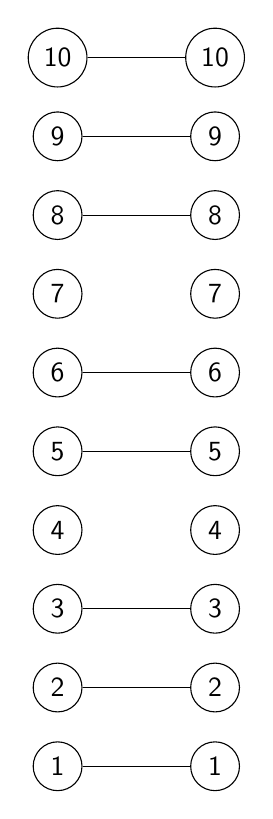
\begin{tikzpicture}
\foreach \x in {1,...,10}
{ \node[circle,draw] (\x 1) at (0,\x) {\x};
	\node[circle,draw] (\x 2)at (2,\x) {\x};
	\ifthenelse{\NOT \x = 4 \AND \NOT 7 = \x}{\draw (\x 1) -- (\x 2);}{}
}
\end{tikzpicture}

\section{Better graphics package for \texttt{includegraphics}}
Like avoid showing file name in graph\\
Solve space in filename issue\\
\texttt{\\usepackage\{grffile\}}

\section{Indent env.}
\begin{verbatim}
\usepackage{enumitem}
\end{verbatim}
\setlist[description]{leftmargin=\parindent,labelindent=\parindent}
left aligned text
\begin{description}
	\item[One] first item
	\item[Two] second item
	\item[Three] third item
	\end{description}

\end{document}